\documentclass[11pt]{article}
\usepackage{amsmath}
\usepackage{amssymb}
\usepackage{microtype}
\usepackage[english]{babel}
\usepackage[labelsep=period, font=small]{caption}
\usepackage[margin=3cm]{geometry}
\usepackage{graphicx}
\usepackage[utf8]{inputenc}
\usepackage{listings}
\usepackage{mdframed}
\usepackage{float}
\usepackage{wisjab}
\usepackage{xcolor}
\usepackage{subfig}

\frenchspacing
\DisableLigatures[f]{}
\parindent=20pt

\definecolor{medgreen}{rgb}{0.0, 0.6, 0.0}
\definecolor{reddishmauve}{rgb}{0.6, 0.0, 0.3}
\lstset{language=Python, showstringspaces=false, numberfirstline=false, breaklines=true, numbers=left, stepnumber=1, tabsize=4,
basicstyle=\ttfamily, numberstyle=\tiny, commentstyle=\color{medgreen}\rmfamily, stringstyle=\color{reddishmauve}, keywordstyle=\color{blue}}

\DeclareMathOperator*{\argmin}{arg\,min}
\DeclareMathOperator*{\argmax}{arg\,max}
\DeclareMathOperator{\Tr}{Tr}
\DeclareMathOperator{\vsgn}{{\bf sgn}}
\def\tab{\hspace*{1cm}}

\author{Anonymous [s\,$*******$] and Unknown [s\,$*******$]}
\title{\textsc{\Huge neural networks}\\Assignment I}

\begin{document}
\maketitle

\section{Introduction}

An artificial neural network is a computational model that is inspired by the way biological nervous systems, like the human brain, process information. The key element of this model is the structure of the information processing system. An artificial neural network uses a number of highly interconnected processing elements (neurons) which process information by their dynamic state response to external inputs. Artificial neural networks learn, just like biological ones, by example. A trained neural network can be considered an expert in the category of information it has been given to analyse.\par
Neural networks can be used to determine patterns and detect trends that are difficult to be noticed by humans or other computer techniques. Since the beginning of neural network development, there have been many breakthrough results in computer vision, speech recognition and text processing.\par
For this assignment, we develop and evaluate several algorithms for classifying images of handwritten digits. We used a simplified version of the MNIST data set\cite{mnist} that consists of a collection of 2707 digits represented by vectors of 256 numbers that represent $16\times16$ images. 
We implement several simple classifiers to classify these images, and compare these with neural network methods. In sections 2 and 3, we turn our attention to classification based on similarity in terms of hyperspace distance between samples. In section 4, we describe a Bayes' rule classifier. In sections 5 and 6, we investigate the performance of actual neural network approaches, including our own implementation of a multi-class perceptron algorithm.

\section{Analysis of distances between images}
For each digit $i$, $i\in\{0, 1, \ldots, 9\}$, let us consider a set of points in 256-dimensional space, $S_i$, which consists of all training images (vectors) that represent the digit $i$. Then, for each set $S_i$, we can calculate its centre $S_i$, and its radius $r_i$, which is defined as
\begin{align}
r_i=\max_{v\in S_i}d(v, S_i),
\end{align}
\begin{table}
\centering
\small
\begin{tabular}{c|cccccccccc}
$i$&0&1&2&3&4&5&6&7&8&9\\\hline
$n_i$&319&252&202&131&122&88&151&166&144&132\\
$r_i$&15.89&9.48&14.17&14.74&14.53&14.45&14.03&14.91&13.71&16.14
\end{tabular}
\caption{Cardinality and point centre for each digit set. It is interesting to see that $S_1$ has a strikingly low radius, indicating relatively little variation of all written 1's in the training set.}
\normalsize
\end{table}
where $d$ is a distance function. We use these definitions to develop a simple classifier in the next section, where elaborate on the definition of $d$. For now, we investigate the characteristics of the training set, in order to get an idea of the separarability of the handwritten digits. The number of elements and (Euclidean) radius of each set are shown in table 1.\par
Now let us look at the distances between the centres of each set. These are shown in table 2. The first thing we see is that most distances are notably smaller than the radii as shown in table 1. While one may be tempted to draw the conclusion that the digits are too similar to be classified by any method involving these values (claiming there is too much overlap between the sets), it is worthwhile to keep in mind that the points defining the radius are extrema. That is, a set having a large radius does not necessarily indicate that all or most points are that far away from the centre; it may even be one point deviating while the others are close to the centre. Nevertheless, we can predict from this knowledge that 7 and 9 will be the most difficult to separate, as the distance between those digits is the smallest; in the same fashion, digits 0 and 1 seem to be the easiest to separate.
\begin{table}
\centering
\small
\begin{tabular}{c|cccccccccc}
&$S_0$&$S_1$&$S_2$&$S_3$&$S_4$&$S_5$&$S_6$&$S_7$&$S_8$&$S_9$\\\hline
$S_0$&0&14.45&9.33&9.14&10.77&7.52&8.15&11.86&9.91&11.49\\
$S_1$&14.45&0&10.13&11.73&10.17&11.12&10.61&10.74&10.09&9.93\\
$S_2$&9.33&10.13&0&8.18&7.93&7.91&7.33&8.87&7.08&8.89\\
$S_3$&9.14&11.73&8.18&0&9.09&6.12&9.30&8.92&7.02&8.35\\
$S_4$&10.77&10.17&7.93&9.09&0&8.00&8.78&7.58&7.38&6.01\\
$S_5$&7.52&11.12&7.91&6.12&8.00&0&6.70&9.21&6.97&8.26\\
$S_6$&8.15&10.61&7.33&9.30&8.78&6.70&0&10.89&8.59&10.44\\
$S_7$&11.86&10.74&8.87&8.92&7.58&9.21&10.89&0&8.47&5.43\\
$S_8$&9.91&10.09&7.08&7.02&7.38&6.97&8.59&8.47&0&6.40\\
$S_9$&11.49&9.93&8.89&8.35&6.01&8.26&10.44&5.43&6.40&0
\end{tabular}
\caption{Distances between each set, determined by Euclidean measure.}
\normalsize
\end{table}
\section{Classifying by distances}
Now that we have conducted a training procedure by having the algorithm compute the centres of the sets from the training set, we can use this to construct a simple classifier $C$ based on this approach:
\begin{align}
C(v)=\argmin_{i\in\{0,\ldots,9\}}d(v, S_i).
\end{align}
We can test the performance of this classifier the training and the test set. For both cases, we present the results as a \textit{confusion matrix} F, whose entries $F_{ij}$ contain the percentage of digits $i$ that were classified as $j$. These are shown in tables 3 and 4.
\begin{table}[!t]
\centering
\small
\begin{tabular}{c|cccccccccc}
&$S_0$&$S_1$&$S_2$&$S_3$&$S_4$&$S_5$&$S_6$&$S_7$&$S_8$&$S_9$\\\hline
$S_0$&0.850&0&0&0&0.006&0.013&0.113&0&0.019&0\\
$S_1$&0&1&0&0&0&0&0&0&0&0\\
$S_2$&0.015&0&0.827&0.045&0.045&0.005&0.015&0.020&0.030&0\\
$S_3$&0&0&0.015&0.916&0.008&0.023&0&0.008&0.023&0.008\\
$S_4$&0&0.066&0.008&0&0.779&0&0.025&0&0&0.123\\
$S_5$&0.034&0&0.023&0.034&0.045&0.761&0.034&0.011&0.023&0.034\\
$S_6$&0.066&0.026&0.033&0&0.013&0&0.854&0&0.007&0\\
$S_7$&0&0.024&0&0&0.012&0.012&0&0.843&0.006&0.102\\
$S_8$&0.007&0.014&0.007&0.069&0.014&0.021&0.007&0&0.840&0.021\\
$S_9$&0&0.023&0&0.008&0.076&0&0&0.045&0&0.848
\end{tabular}
\caption{Confusion matrix for the training set, using Euclidean measure.}
\normalsize
\end{table}
\begin{table}
\centering
\small
\begin{tabular}{c|cccccccccc}
&$S_0$&$S_1$&$S_2$&$S_3$&$S_4$&$S_5$&$S_6$&$S_7$&$S_8$&$S_9$\\\hline
$S_0$&0.795&0&0.013&0.009&0.018&0.009&0.103&0.004&0.045&0.004\\
$S_1$&0&0.992&0&0&0&0&0.008&0&0&0\\
$S_2$&0.020&0&0.683&0.059&0.079&0.010&0&0.020&0.129&0\\
$S_3$&0.038&0&0.038&0.772&0.013&0.101&0&0&0.013&0.025\\
$S_4$&0.012&0.035&0.035&0&0.802&0&0.012&0.012&0&0.093\\
$S_5$&0.055&0&0&0.109&0.055&0.691&0.018&0&0&0.073\\
$S_6$&0.078&0&0.022&0&0.022&0.011&0.867&0&0&0\\
$S_7$&0&0.031&0.016&0&0.078&0&0&0.781&0&0.094\\
$S_8$&0.033&0.022&0&0.065&0.033&0.033&0&0&0.793&0.022\\
$S_9$&0&0.057&0&0&0.091&0&0&0.057&0.023&0.773
\end{tabular}
\caption{Confusion matrix for the test set, using Euclidean measure.}
\normalsize
\end{table}
It seems that in the training set, the digit pairs $(0, 6)$, $(4, 9)$ and $(7, 9)$ are the most difficult to separate, as these are misclassified the most often. However, the reverse is not as apparent: for example, 9 is classified as 7 less than half as often as the other way around. The test set shows more symmetric behaviour, in that for example $F_{49}$ is very close in value to $F_{94}$. In addition to the three aforementioned digit pairs, the pair $(3, 5)$ appears to be difficult to separate as well. In the end, the prediction about 7 and 9 being difficult to separate has been confirmed, although there are clearly more difficult pairs, contrary to what the distance matrix suggests.\par
We can measure the overall accuracy $A$, defined as
\begin{align}
A=\overline{\sum_{i=0}^9F_{ii}}=\frac{1}{10}\Tr\mathrm{F}
\end{align}
for different distance functions. We use several distances from \verb|sklearn| Python package. For further details regarding those functions refer to the Scikit-learn documentation\cite{scikit}. The results of this procedure are shown in table 5. We can see that the Euclidean distance and the correlation distance provide the best performance on the test set.
\begin{table}[!t]
\centering
\small
\begin{tabular}{c|cc}
&training set&test set\\\hline
Euclidean&0.852&0.795\\
city block&0.742&0.697\\
cosine&0.850&0.788\\
Bray-Curtis&0.706&0.656\\
Canberra&0.426&0.395\\
Chebyshev&0.823&0.762\\
correlation&0.855&0.795\\
Mahalanobis&0.954&0.678\\
standardised Euclidean&0.840&0.776
\end{tabular}
\caption{Overall accuracies of the distance classifier on the training and test set for different distance functions.}
\normalsize
\end{table}
\newpage
\section{Bayes rule classification}
The Bayes rule classifier is a simple probabilistic classifier that is based on Bayes' theorem with strong independence assumptions between features of different classes. To keep things simple we will limit ourselves to two classes, $S_1$ and $S_9$. The feature we considered was the amount of white space ($X$) contained in the images corresponding to these classes.\par
In order to determine what class an image belongs to one would, without any knowledge about the value of $X$, choose $S_1$ if $P(S_1)>P(S_9)$ and choose $S_9$ otherwise. If we do know the value of $X$ however, we will need to estimate the probabilities $P(S_1|X)$ and $P(S_9|X)$ which we can calculate with Bayes' theorem. This theorem states that
\begin{align}
P(S_i|X)=\frac{P(X|S_i)P(S_i)}{P(X)}.
\end{align}
By plotting a histogram of the data belong to the two classes we can calculate these probabilites. Such a histogram is shown in figure 1.
\begin{figure}[!b]
\centering
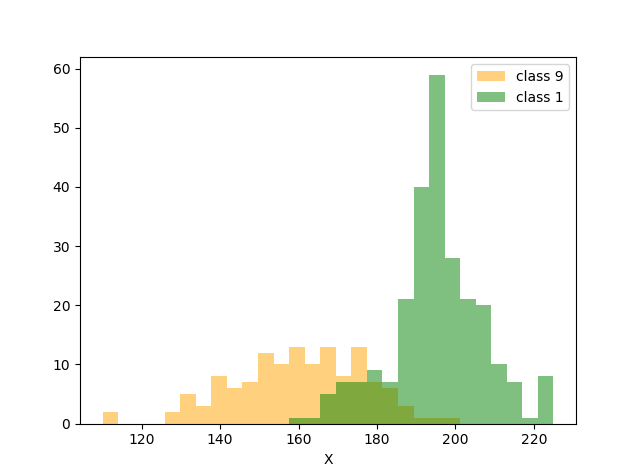
\includegraphics[width=0.68\textwidth]{histogram1_9.png}
\caption{Occurence of instances with different amounts of whitespace (labelled by $x$) belonging to classes $S_1$ and $S_9$.}
\end{figure}
With this method, we can define the following empirical probabilities:\vspace*{2mm}
\begin{align}
&P(X|S_i)=\frac{N(X, S_i)}{N(S_i)},\\[2mm]
&P(S_i)=\frac{N(S_i)}{N},\\[2mm]
&P(X)=\frac{N(X)}{N},
\end{align}
where $N(S_i, ...)$ is the number of samples belonging to class $S_i$, $N(..., X)$ is the amount of samples in the whitespace interval $X$, and $N$ is the total number of samples. Taking this all into account we simply arrive at
\begin{align}
P(S_i|X)=\frac{N(X, S_i)}{N(X)}
\end{align}
The classifier then checks, for every image that falls into the whitespace interval $Y$, which of the probabilities $P(S_i|Y)$ and $P(S_j|Y)$ is largest, and classifies it as the set with the largest probability. The probabilites have been calculated from the training set for the classes 1 and 9. Subsequently, the training set and test set have been classified with the Bayes classifier resulting in the accuracies shown in table 6.\par
\begin{table}[t]
\centering
\small
\begin{tabular}{c|cc}
class&training set&test set\\\hline
1&0.916&0.859\\
9&0.848&0.761\\
\end{tabular}
\caption{Accuracies of the Bayes rule classifer on the training and test set for classes 1 and 9.}
\normalsize
\end{table}
These accuracies seem quite high for such a weak feature. This is because class 1 has much less white space than any other of the classes. So it results into a well defined feature. Of course, this is not the case if we choose any other pair of classes that do not contain class 1. For example, when we try to classify the classes 2 and 9 and the classes 4 and 6 we get the accuracies in tables 7 and 8.
We see that the accuracy of our classifier becomes significantly worse, indicating that the amount of whitespace is not a well defined feature for classes that do not have a large difference between their whitespace.
\begin{table}[!h]
\centering
\small
\begin{tabular}{c|cc}
class&training set&test set\\\hline
2&0.757&0.703\\
9&0.575&0.636
\end{tabular}
\caption{Bayes rule classification accuracies for classes 2 and 9.}
\normalsize
\end{table}
\begin{table}[!h]
\centering
\small
\begin{tabular}{c|cc}
class&training set&test set\\\hline
4&0.262&0.174\\
6&0.901&0.911
\end{tabular}
\caption{Bayes rule classification accuracies for classes 4 and 6.}
\normalsize
\end{table}
\section{Perceptron algorithm}
Now we turn to a neural network approach in hopes of creating a better classifier than the ones implemented in the previous parts. More specifically, we implement a perceptron network: a neural network with one input layer of 256 nodes, one output layer of 10 nodes (one for each digit) and no hidden layers. The weights and the biases of the output nodes are initialised randomly according to a uniform distribution over the interval $[0, 1)$. For each output digit $n$, we make use of an \textit{check vector} $\vc{c}$ such that $c_m=2\delta_{mn}-1$, with $\delta$ the Kronecker delta symbol. In order to train the network, we execute the following procedure:\\
\sf
\begin{mdframed}
$\eta:=\text{learning rate}$\\
$\mt{W}:=\text{randomly initialised }10\times256\text{ weight matrix}$\\
$\vc{w}_b:=\text{randomly initialised } 10\times1\text{ bias vector}$\\
\textbf{for} $i=1..\text{number\_of\_epochs}$ \textbf{do}\\
\tab\textbf{for} $j=1..\text{training\_set\_size}$ \textbf{do}\\
\tab\tab$\vc{x}:=j\text{-th input vector}$\\
\tab\tab$\vc{c}:=j\text{-th output vector}$\\
\tab\tab$\vc{a}:=\vc{w}_b+\mt{W}\vc{x}$\\
\tab\tab$\vc{y}:=\vsgn(\vc{a})$\\
\tab\tab$\mt{W}:=\mt{W}+\eta(\vc{c}-\vc{y})\vc{x}\T$\tab\#~$\vc{x}\T$ is a row vector\\
\tab\tab$\vc{w}_b:=\vc{w}_b+\eta(\vc{c}-\vc{y})$\\
\tab\textbf{end}\\
\textbf{end}
\end{mdframed}$ $\\
\rm
The digit as which an input vector $\vc{x}$ is classified, is then
\begin{align}
C(\vc{x})=\argmax_{i\in\{0,\ldots,9\}}a_i,
\end{align}
where $\vc{a}$ is the output vector as used in the algorithm listed above.\par
We train the perceptron network for different numbers of epochs, after which we evaluate the performance of the network on both the training set and the test set. We use a learning rate $\eta=5$. The results are shown in figure 2. We see that the training time mainly affects the accuracy on the training set, which is to be expected, given the characteristics of such a network. On the other hand, the accuracy on the test set seems to improve by a mere 2-3 per cent as we increase the training time from a few epochs to 50 epochs. Something that could explain this is the relatively low complexity (that is, 2570 connections) compared to the number (1707) of training instances used to train the network. As such, the network becomes fully trained quite quickly in terms of the number of epochs, which translates to seemingly small improvement as seen in the figure.\par
What's more is that the perceptron network seems to achieve a 100 per cent accuracy on the training set, which indicates that the training set is tenfold linearly separable, which is something one might not expect at first glance. This is remarkable, as recognition of handwriting is in general a difficult task---even we humans cannot do it perfectly at all times.
\begin{figure}[!t]
\centering
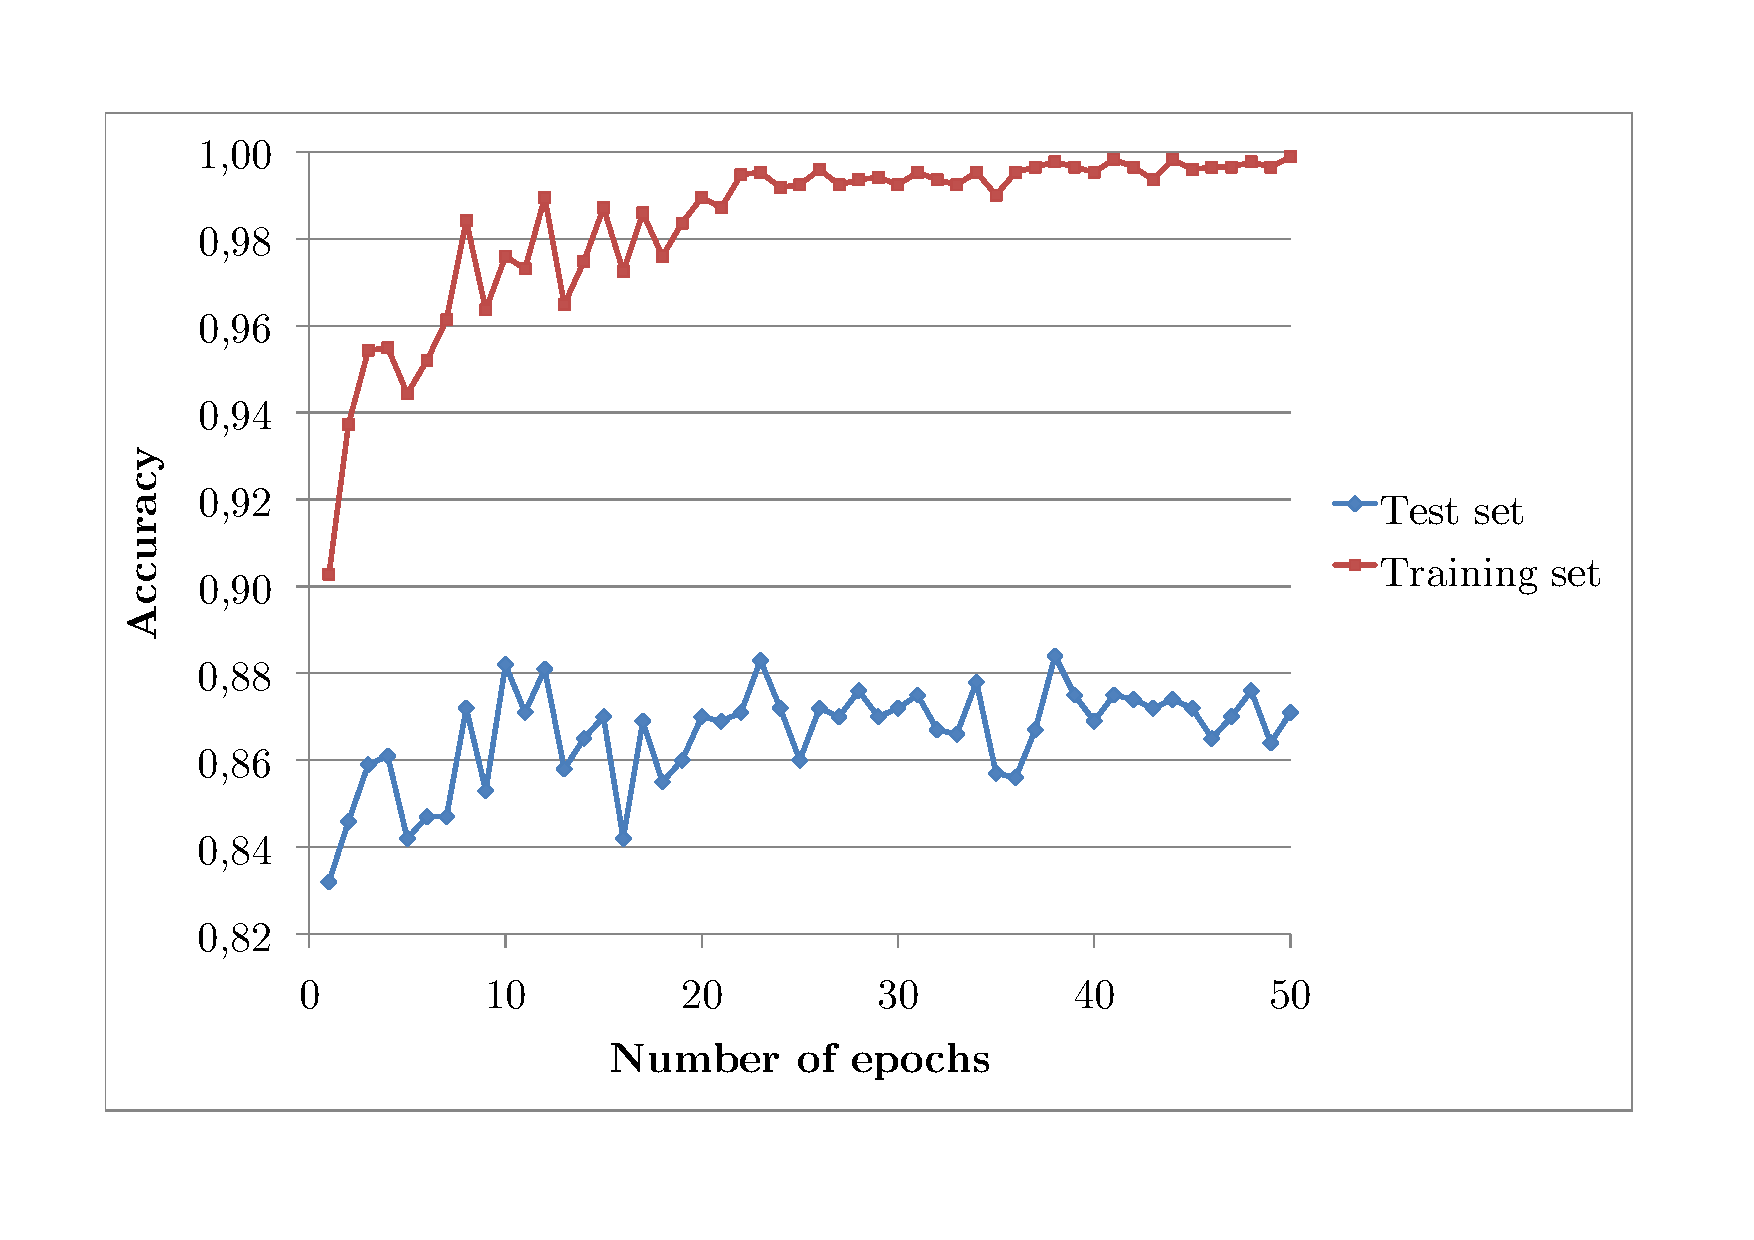
\includegraphics[width=0.85\textwidth]{O1_4_epochs.pdf}
\caption{Performance of the perceptron algorithm on both the training set and test set, for a different number of epochs.}
\end{figure}
\section{Model checking with existing software}
So far we have used simple classifiers achieving accuracy results up to 80\%. Then we turned to a neural network approach by implementing the perceptron algorithm and achieved an accuracy of 100\% on the training set, and an accuracy of up to 88\% on the test set.\par
Now we want to use a more advanced neural network to compare our classifiers with. For this task, we have used Michael Nielsen's code from his book \textit{Neural networks and deep learning}\cite{nndl}. This network learns the weights and biases from a gradient descent backpropagation method, repeately applied to smaller subsets or \textit{mini-batches} of the data set. This method is also known as \textit{stochastic gradient descent}. In order to test the performance of this algorithm, we compare its accuracy on the training and test set while varying different parameters and using different network topologies. The parameters that we consider are the learning rate $\eta$, and the mini-batch size $m$. Since it is in general a challenging task to find the optimal parameters of a neural network (we could even write a neural network to do just that), we try to find good values for these parameters heuristically. That is, we tune each property one by one while fixing the others and see how the network behaves.\par
For example, we can start with a network that has one hidden layer (in addition to the 256-node wide input layer and the 10-node wide output layer) of $n=30$ neurons, a learning rate $\eta=10$ and a mini-batch size $m=50$. The accuracy of this network, as a function of the number of epochs used to train the network, is shown in figure 3.\par
\begin{figure}[!t]
\centering
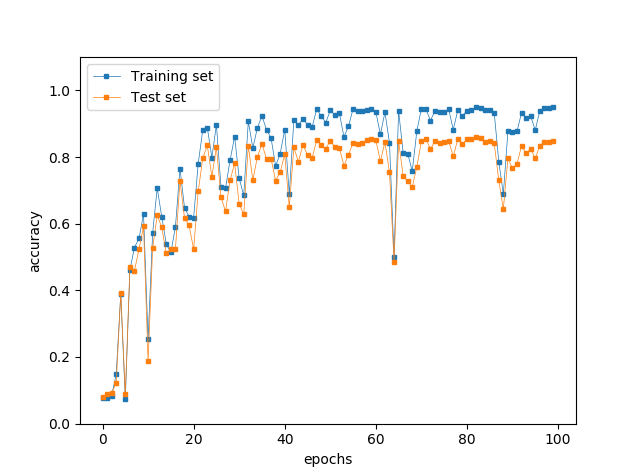
\includegraphics[width=0.6\textwidth]{accuracies_example.png}
\caption{Accuracy on the training and test set, with one 30-node wide hidden layer, $\eta=10$ and $m=50$.}
\end{figure}
\begin{figure}[!b]
\centering
\parbox{6cm}{
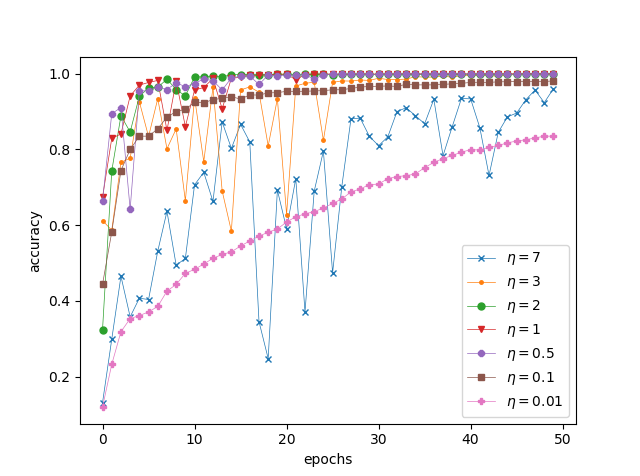
\includegraphics[width=7.5cm]{delta_eta_train.png}
\caption{Accuracy on the training set, varying $\eta$, $n=30$, $m=50$.}
}
\qquad
\begin{minipage}{6cm}
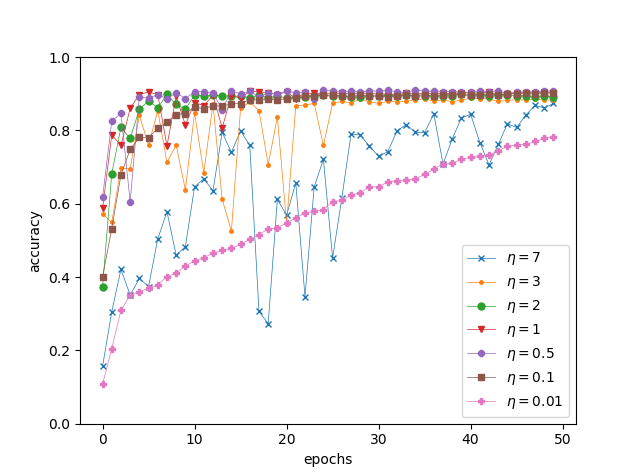
\includegraphics[width=7.5cm]{delta_eta_test.png}
\caption{Accuracy on the test set, varying $\eta$, $n=30$, $m=50$.}
\end{minipage}
\end{figure}
Although the accuracies slowly tend to a level higher than 80\%, there seem to be a lot of jumps. This unstable behaviour could well be caused by a learning rate that is too high. To see if this assumption is correct, we repeat the experiment for different values of $\eta$, while keeping $m$ constant, and check whether the results improve or not. This is shown in figures 4 and 5. We see that the learning rates around $\eta=1$ yield the best performance, converging quickest to 100\% on the training set, and about 90\% on the test set. As expected, learning rates closer to 10 produce more whimsical learning curves. Furthermore, low learning rates ($\eta=0.01$) make the network weights converge to the optimum very slowly.\par
Subsequently, we take $\eta=1$, and we check the performance for different mini-batch sizes (see figure 6 and 7). We see that mini-batch size around $m=10$ gives quite a good accuracy. What helps us interpret and understand these results is the fact that the smaller $m$ is, the more often the gradient descent rule is altered according to the output error---after all, the same update rule (in term of error vectors) is applied for all instances in one mini-batch. As such, a mini-batch size that is too small will inevitably cause the network to get stuck in local minima.\par
\begin{figure}[!t]
\centering
\parbox{6cm}{
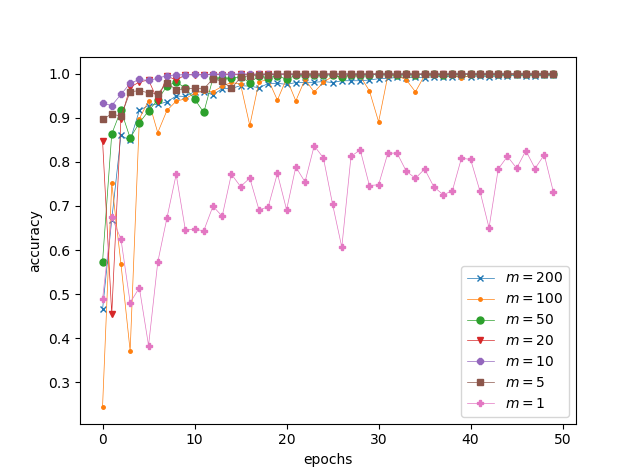
\includegraphics[width=7.5cm]{delta_m_train.png}
\caption{Accuracy on the training set, varying $m$, $n=30$, $\eta=1$.}
}
\qquad
\begin{minipage}{6cm}
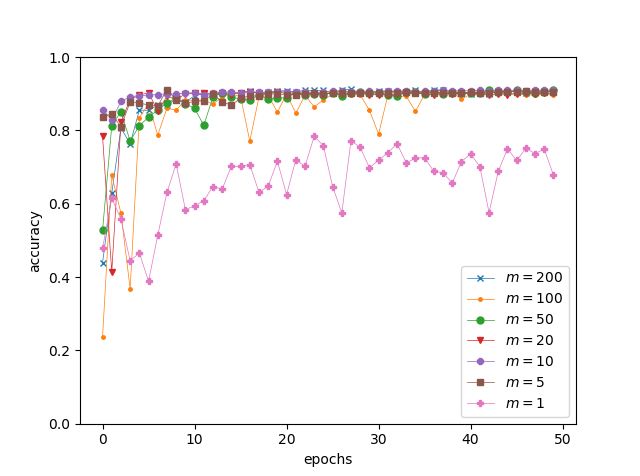
\includegraphics[width=7.5cm]{delta_m_test.png}
\caption{Accuracy on the test set, varying $m$, $n=30$, $\eta=1$.}
\end{minipage}
\end{figure}
\begin{figure}[!b]
\centering
\parbox{6cm}{
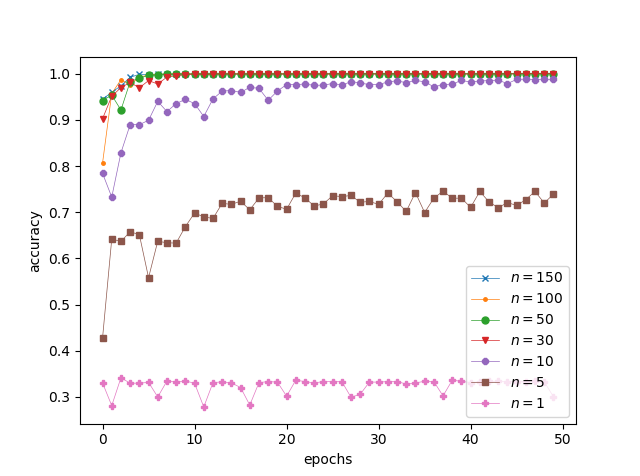
\includegraphics[width=7.5cm]{delta_n_train.png}
\caption{Accuracy on the training set, varying $n$, $m=10$, $\eta=1$.}
}
\qquad
\begin{minipage}{6cm}
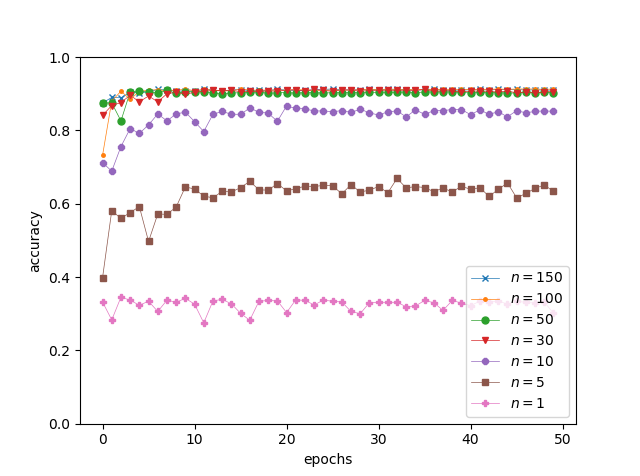
\includegraphics[width=7.5cm]{delta_n_test.png}
\caption{Accuracy on the test set, varying $n$, $m=10$, $\eta=1$.}
\end{minipage}
\end{figure}
Now we look at the influence that the width of the hidden layer has on the performance of the network. We set $m=10$ and $\eta=1$, and vary the number of nodes in this layer. See figures 8 and 9. It seems that the accuracy is optimal for a neuron number around 100 and increasing this does not seem to effect the accuracy of the network. At this number of nodes, the separation curve is `smoothed out' enough, and adding more to smoothen it even further has no observable effect. The highest accuracy we were able to achieve on the test set was for $\eta=1.2$, $m=10$ and $n=100$ with an accuracy of 91\%.\par
Lastly, we consider the number of hidden layers. Given the fact that adding new layers severely affects the shape of the separation curve, one would expect visibly different behaviours for different amounts of layers. The impact on the accuracies (both training and test set) of varying the network topology in this fashion is shown in figures 10 and 11. We immediately see that increasing the number of layers of the network dramatically decreases the accuracy. While this is not very surprising for the test set---indeed, one would expect huge overfitting to occur at high network depths---, it is somewhat strange to see the accuracy on the test set plummet with increasing depth as well. One reason that we could give for this is that the separation curve becomes unnecessarily complex, and starts in such a messy configuration that it would take ages to properly adjust it---if we can even fix it at all. Clearly, the optimal number of hidden layers is one, which is what we started with in the first place.
\begin{figure}[!t]
\centering
\parbox{6cm}{
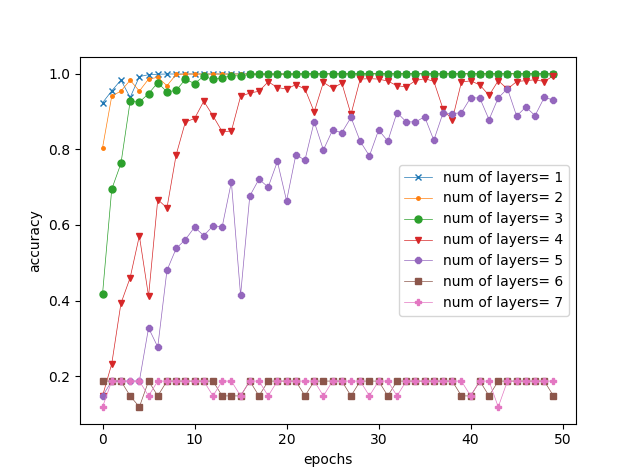
\includegraphics[width=7.5cm]{delta_layers_train.png}
\caption{Accuracy on the training set, varying number of layers, $n=100$, $m=10$, $\eta=1$.}
}
\qquad
\begin{minipage}{6cm}
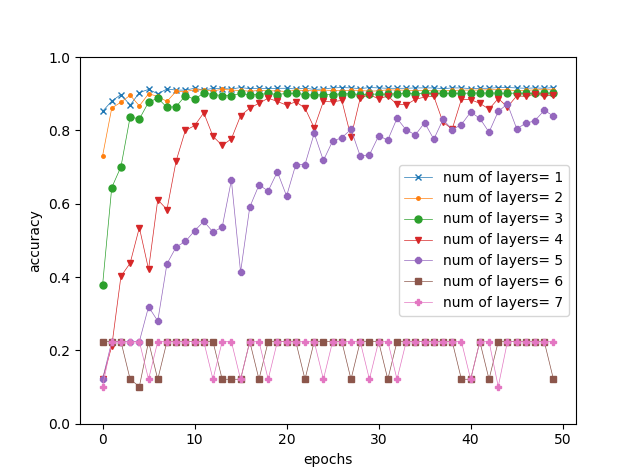
\includegraphics[width=7.5cm]{delta_layers_test.png}
\caption{Accuracy on the training set, varying number of layers, $n=100$, $m=10$, $\eta=1$.}
\end{minipage}
\end{figure}
\vspace*{\fill}
\begin{thebibliography}{x}
\bibitem{mnist}Yann LeCun, Corinna Cortes, Christopher J.C. Burges, \textit{The MNIST database}. Url:\\
\verb|http://yann.lecun.com/exdb/mnist|
\bibitem{scikit}\textit{Scikit-learn: machine learning in Python}. Url:\\
\verb|http://scikit-learn.org/stable/modules/generated/sklearn.metrics.|\\\verb|pairwise.pairwise_distances.html|.
\bibitem{nndl} Michael Nielsen, \textit{Neural networks and deep learning}. Url:\\
\verb|http://neuralnetworksanddeeplearning.com/index.html|
\end{thebibliography}
\end{document}
